\documentclass[12pt,a4paper,titlepage]{article}
\usepackage[latin1]{inputenc}
\usepackage{amsmath}
\usepackage{amsfonts}
\usepackage{amssymb}
\usepackage{makeidx}
\usepackage{graphicx}
\usepackage{subcaption}

\makeatletter
\setlength{\@fptop}{0pt}
\makeatother

\oddsidemargin 1cm
\evensidemargin 1cm
\textwidth 15cm
\topmargin -1.25cm
\textheight 24.37cm

\renewcommand{\listfigurename}{Figures}
\renewcommand{\listtablename}{Tables}

\begin{document}	
	\begin{titlepage}
		\begin{figure}
			
\includegraphics[width=.6\linewidth]{images/logoWWU}
		\end{figure}
		\vspace*{2cm}
		\begin{center}
			Title:\\			
			\textbf{Application of Data Analytics in Failure Pattern Recognition}
			
			\vspace*{3cm}
			\textbf{Seminar Thesis}\\			
			In the context of the seminar ``Application of Data Analytics in Spare Parts Supply Chain Management''\\
			at the Chair for Information Systems and Supply Chain Management
		\end{center}
		\vspace*{1.5cm}
		\begin{tabbing}
			\hspace*{4cm}\= \kill
			Supervisors:			\> Dr.-Ing.Christian Grimme\\
									\> Dipl.-Inf. Jakob Bossek\\
									\> Carolin Wagner MScIS\\
			\\
			Presented by:			\> Alexander Anokhin\\
									\> Busso-Peus-Str. 14\\
									\> Muenster 48149\\
									\> Germany\\
									\> +4917675615943\\
									\> a\_anok01@uni-muenster.de\\
									\\
									\> Joshua Peter Handali\\
									\> Street\\
									\> Muenster zip-code\\
									\> Germany\\
									\> Mobile Phone\\
									\> j\_hand01@uni-muenster.de\\
			\\
			Date of submission: 	\> \today\\
		\end{tabbing}
	\end{titlepage}	
	
	\pagenumbering{gobble}
	\tableofcontents
	\newpage	
	
	\pagenumbering{Roman} 
	\setcounter{page}{1}
	\clearpage
	
	\addcontentsline{toc}{section}{Figures}
	\listoffigures
	\newpage
		
	\addcontentsline{toc}{section}{Tables}
	\listoftables
	\newpage
	
	\section*{Abbreviations}
	\addcontentsline{toc}{section}{Abbreviations}
	\begin{tabbing}
		\hspace*{3cm}\= \kill
		ANN				\> Artificial Neural Networks\\
		CART			\> Classification and Regression Trees\\
		SVM				\> Support Vector Machine\\		
	\end{tabbing}
	\newpage
	
	\pagenumbering{arabic} 
	\setcounter{page}{1}
	\section*{Introduction 1 page}
	\label{introduction}
	\addcontentsline{toc}{section}{Introduction}
	\textbf{SVM Reminder} Support vector machine (SVM) is a relatively new computational learning method based on the statistical learning theory. Exhaustive overviews of SVM applicability in pattern recognition \cite{Lee2002} and fault diagnosis \cite{Widodo20072560} clearly show that SVM is a versatile and efficient technique for such problems. The concept of SVM is based on Vapnik-Chervonenkis theory \cite{cortes1995support, vapnik1995nature} that recently emerged as a general mathematical framework for estimating (learning) dependencies from finite samples \cite[p. 2561]{Widodo20072560}. The idea of SVM is to separate feature space by constructing linear boundaries between two classes. Moreover initial feature space can be enlarged with help of kernel transformations. 
		
	SVM approach is not only theoretically well-founded, but also superior in practice. Recent surveys show that tuned SVM classifiers has become more efficient in pattern recognition than other methods: Artificial Neural Networks (ANN) \cite{Deng20116007, Jodas2013240, Kamruzzaman2006, pan2012parkinson, Shao201278} and Classification and Regression Trees (CART) \cite{marnerides2015fault, Shao201278}. In addition, SVMs have one significant advantage compared to conventional methods of pattern recognition such as ANNs. These methods straggle to solve problems with a small number of samples. For the reason that it is hard to obtain sufficient fault samples in practice, SVM is introduced into machines fault diagnosis due to its high accuracy and good generalization for a smaller number of samples \cite[p. 2562]{Widodo20072560}. 
	
	\section{Problem Description 1.5-2 pages}
	\subsection{Research Methodology}
	\textbf{Aim and Research Questions} Aim of analysis is to build a classifier, based on initially collected data, to detect failures. Such a diagnosis can highly benefit company in real life, since failures identified at early stage future costly faults possibly prevented. The aim defines a number of research questions. First of all, it is unclear how the initially proposed data can be properly preprocessed. Moreover, since classes are possible unbalanced another question is how they can be balanced and should they be balanced at all. Since feature extraction and selection as well as SVM parametrization are highly effect final results it will be also valuable to answer the question about optimal procedure and parameters. Another question is how accuracy and efficiency of a classifier can vary along different settings, for example size of initial sample. 
	
	\textbf{Research Design} To accomplish the aim of a study research design was mainly based on optimization and simulation experiments, however literature research was also used in two ways: establish a proper direction of analysis; identify for further use existing methods and approaches. Analysis was conducted with help of R programming language\footnote{http://www.r-project.org/} which was used for statistical computing and graphics.
	
	\subsection{Data Description}
	\textbf{Experiment Set-Up} The initial data is provided by a Brazilian manufacturer. The company produces different kinds of	electric actuators to drive control values. Data are generated in a test environment under normal and overload conditions. Three sensors are installed near the
	gears that are able to record the incurring vibration. The test environment is depicted at Figure \ref{fig:testEnvironment}. Sensor 1 is located in the bearing of the main spindle, Sensor 2 on the motor's bearing and Sensor 3 depicts a built-in torque sensor.
		
	\begin{figure}[h!]
		\centering
		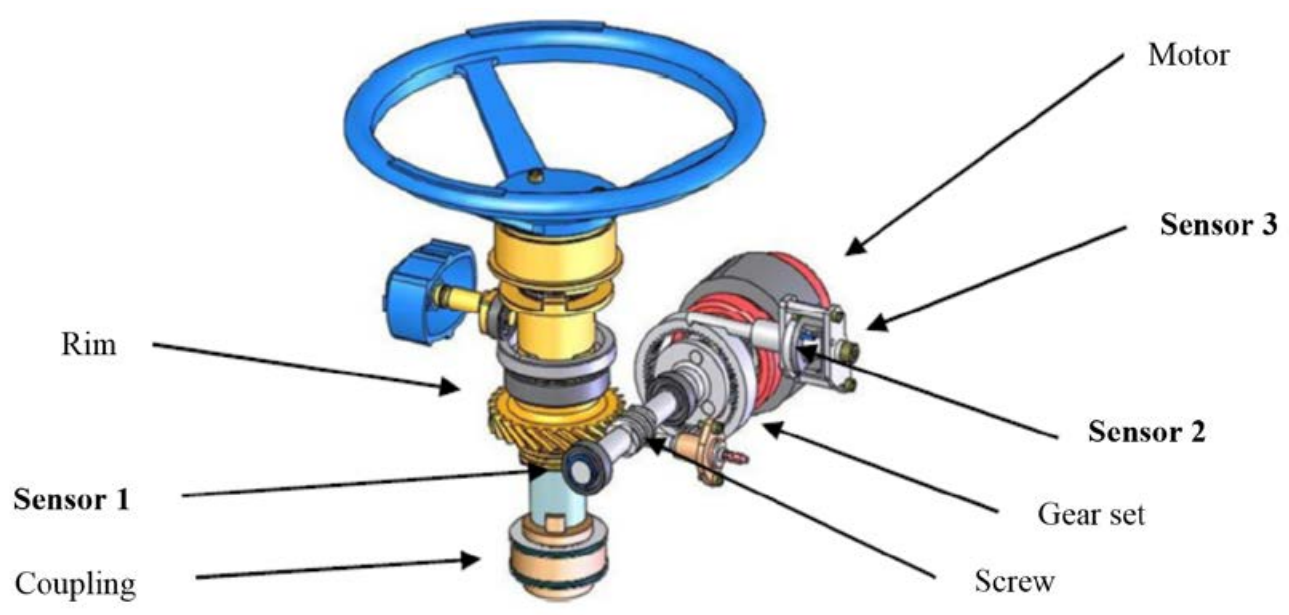
\includegraphics[width=1\linewidth]{images/testEnvironment}
		\label{fig:polinom}
		\caption{Test Environment}
		\label{fig:testEnvironment}
	\end{figure}	  
	
	Tests perform valve aperture actions and are initiated under different conditions. New gears are	considered with and without additional load. In addition, failure data is obtained using worn and broken gears therefore provided data comprises six different settings with three types of failures. For every second is collected 2048 observations of signal. Each cycle lasts about 46-47 seconds. Table \ref{table:generatedData} summarizes generated data.
	
	\begin{table}[h!]
		\centering
		\begin{tabular}{ | l | l | c | c | }
			\hline
			\multicolumn{1}{ | c | }{\textbf{Class}} 
				& \multicolumn{1}{ | c | }{\textbf{Description}}
				& \multicolumn{1}{ | c | }{\textbf{Cycles}} 	
				& \multicolumn{1}{ | c | }{\textbf{Observations}}\\
			\hline
			Normal 1 	& Cycle without load on actuator 			& 25 		& $2398*10^3$\\
			Normal 2 	& Cycle with pressure equal 3.0 bar 		& 25 		& $2572*10^3$\\
			Normal 3 	& Cycle with pressure equal 1.0 bar 		& 25 		& $2392*10^3$\\
			Failure 1 	& Cycle with a worn gear without load 		& 10 		& $930*10^3$\\
			Failure 2 	& Cycle with two worn gears without load 	& 2 		& $195*10^3$\\
			Failure 3 	& Cycle with a broken gear without load 	& 10 		& $946*10^3$\\
			\hline
		\end{tabular}
		\caption{Generated Data} 
		\label{table:generatedData}
	\end{table}
	
	Table \ref{table:generatedData} outlines three important aspects of further analysis. First, provided data are highly unbalanced along classes. The most unbalance case is between Normal 2 and Failure 2 classes. The unbalance ratio here accounts for 75:1000. Second, generated data consist of about 10 millions observations in total which makes computationally impossible to use SVM directly. Third, slightly more emphasis in analysis is putted on comparison of Normal 1 and failure classes since they have been all obtained without load. That is premised in assumption of being able to measure load directly. Since load is measured we can explicitly exclude classes with or without load depending on estimated load. 
	
	\section{Data Preparation 1.5-2 pages}
	\subsection{Data Preprocessing}
	\subsection{Exploratory Analysis}
	
	\section{Data Balancing 3 pages}
	
	\section{SVM Classifier 3.5-4 page}
	
	\section{Results and Discussion 1-1.5 page}
	
	\section{Conclusion 0.5 page}
	
	
	\bibliographystyle{plain}
	\bibliography{References}
	\newpage
	
	\section*{Declaration of Authorship}
	We hereby declare that, to the best of our knowledge and belief, this Seminar Thesis titled ``Application of Data Analytics in Failure Pattern Recognition'' is our own work. We confirm that each significant contribution to and quotation in this thesis that originates from the work or works of others is indicated by proper use of citation and references.
	\\\\	
	M�nster, \today
		
\end{document}